
\section{Design - Static Diagrams}

\begin{figure}[]
\center
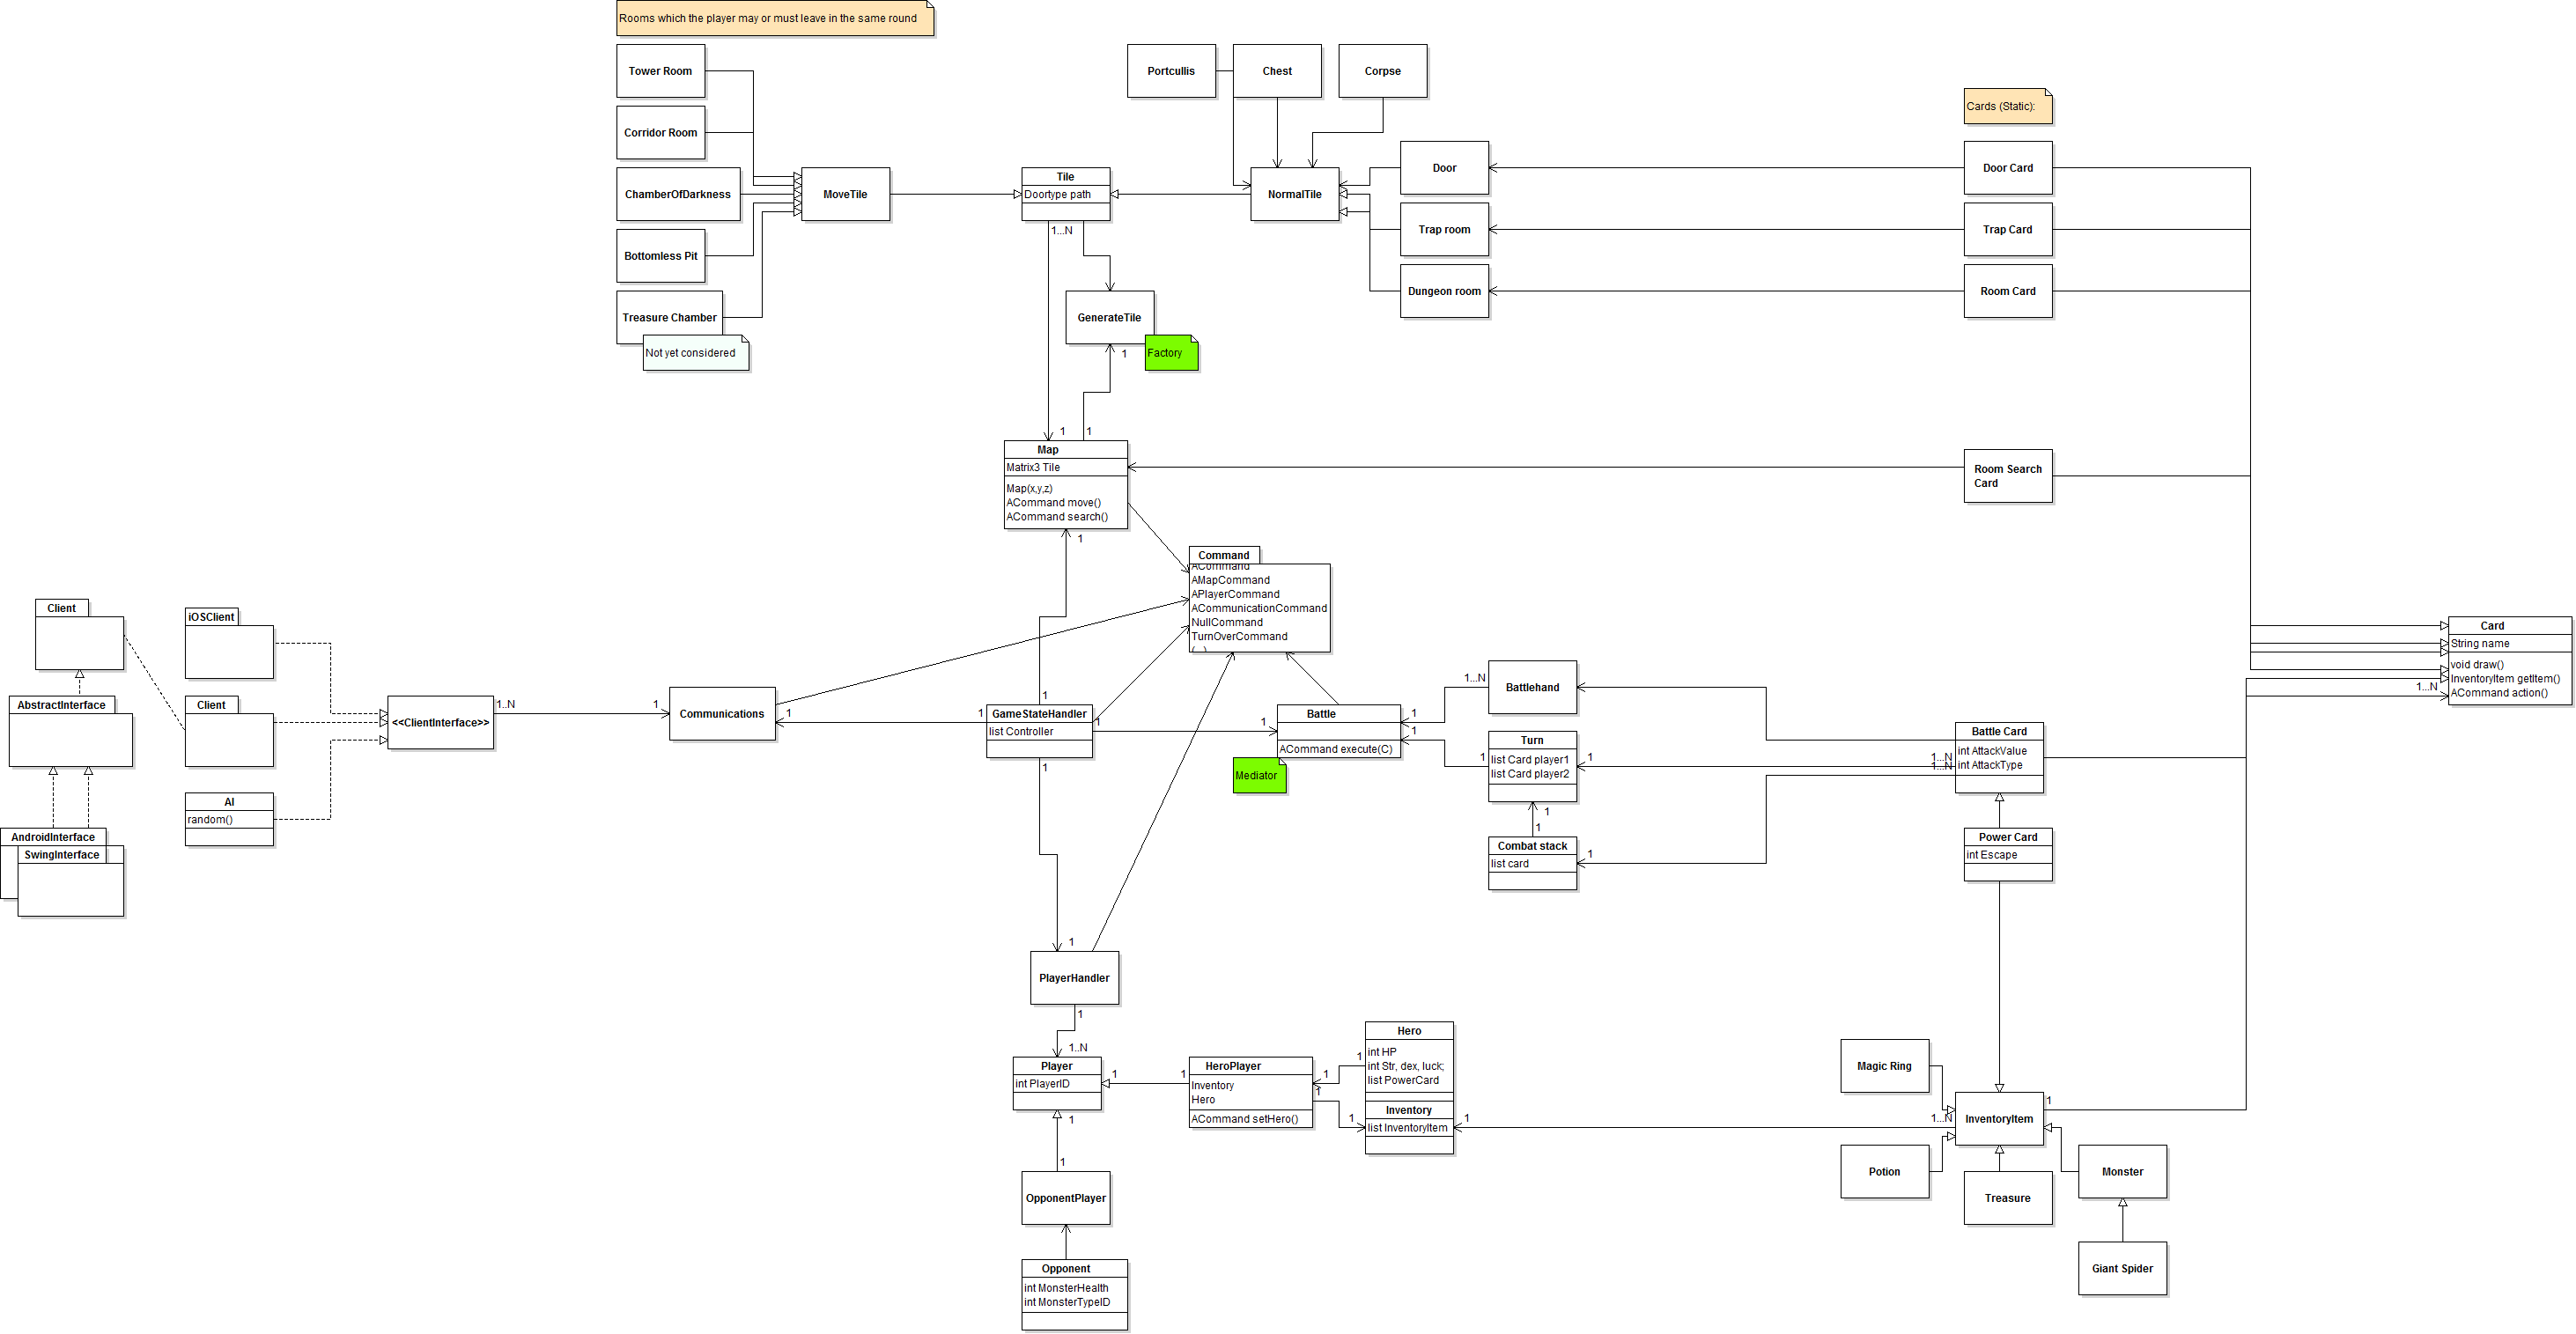
\includegraphics[width=1.65\textwidth,angle=90] {diagrams/ClassDiagram.png}
\caption{Incomplete class diagram.}
\label{classdiagram}
\end{figure}


\begin{figure}[]
\center
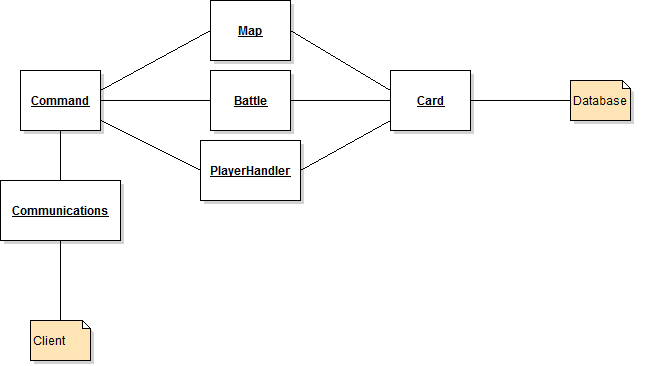
\includegraphics[width=0.9\textwidth] {diagrams/ArchitectureDiagram.png}
\caption{Architecture diagram of the project.}
\label{architecture}
\end{figure}


The game is designed to be a multi-platform, multi-player game, available to a multitude of platforms. In order to achieve this, the game is written in the JAVA programming language, which is supported by all major platforms available today, with the exception of the iOS. To make the game available to also to the iOS, an additional client need be written in Objective-C. By moving most game logic to the server side, the cost and effort required to design the clients is reduced. Clients are only responsible for the graphical representation of the game, and may represent the gamestate in varying ways as long as the communication between the server and the client follows the communication API, which at this point of the design has not yet been decided upon. This also allows for user-generated clients to be designed. In figure \ref{architecture}, the server-client structure is represented by the line connecting \texttt{client} and \texttt{communications}.

The diagram in figure \ref{architecture} describes different packages within the game illustrated by white boxes, and additionally communication with external information sources, \texttt{client} and \texttt{database}. All classes seen in figure \ref{classdiagram} are part of one of the packages in the architecture diagram, see section \ref{packagestructure} for the exact distribution.


\subsection{Command Package}
The \texttt{command} package is in some sense the heart of the system implementation. All communication between packages (the \texttt{Card} package excluded) goes through the \texttt{command} package as a relay, which keeps the coupling low within the system. The \texttt{GameStateHandler} class has the main responsibility of executing commands, and is able to do so without any knowledge of the nature of the command it executes. As long as there are commands on the command stack, they will be executed until a \texttt{TurnOverCommand} is received, on which point the \texttt{GameStateHandler} sends a query to the player whose turn it is.

When a subsystem needs to send a request or invoke an action in another subsystem, it will generate a command of a type that is destined for the subsystem in question. There are four types of abstract commands, \texttt{MapCommand}, \texttt{CommunicationCommand}, \texttt{PlayerCommand} and \texttt{BattleCommand}, with the destination subsystems as indicated by the names. Each of these command types have concrete commands connected to them, an overview of the (not yet complete) structure of the commands can be see in figure \ref{commandstructure}.

Note that subsystems do not send commands to the \texttt{GameStateHandler}, but rather respond to calls from the \texttt{GameStateHandler} with new commands, and all commands always respond with a new command with the exception of the \texttt{NullCommand} and the \texttt{TurnOverCommand}. An example of this can be seen in figure \ref{commandsequence}.

An implication of this structure is that the rules of the game are not highly coupled with the game, instead residing in the ‘’leaves’’, in most cases the Cards. Cards all have a Command connected to them and receiving a card will cause that command to be invoked. Adding new rules to the game will then often be as easy as to add a new type of card to the game. As an example, say a card would be added that allows the player to move an additional time during his/her round, a card that can be found when searching a room. This would be implemented by adding a new card of the type \texttt{SearchCard}, which generates a \texttt{MoveQueryCommand} (does not yet exist), and no other changes to the program would be needed.


\begin{figure}[]
\center
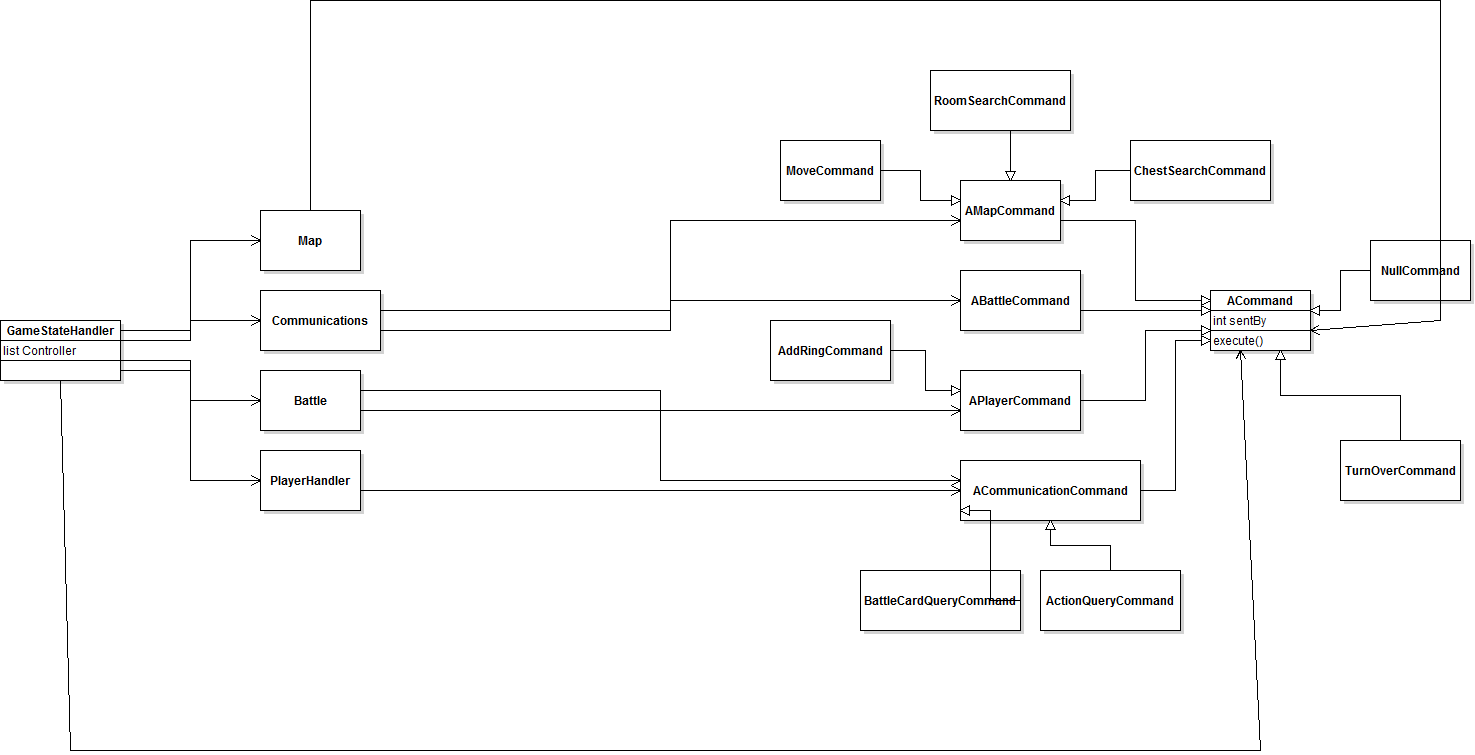
\includegraphics[width=0.9\textwidth] {diagrams/CommandStructureDiagram.png}
\caption{Structure of Commands.}
\label{commandstructure}
\end{figure}


\subsection{Package Structure}
\label{packagestructure}
\begin{itemize}
\item
Map (package)
	\begin{itemize}
	\item
	Map (class) - Map is responsible for keeping track of the game board, positions of players and includes methods to perform actions on the map, such as \texttt{move}.
	\item
	GenerateTile - GenerateTile is responsible for creating a new random Tile, that makes sense in its current position (doors do not lead into walls for example).
	\item
	Tile - abstract class for tiles, the different concrete subclasses define what kind of tile that is generated by GeneraTetile. Each subclass encapsulates 	 tile specific information.
	\end{itemize}
\item
Battle (package)
	\begin{itemize}
	\item
	Battle (class) - Battle is a mediator (see Mediator design pattern) in the battle sequence and makes sure it calls the correct objects involved in the battle.
	\item
	Battlehand - Each player involved in the battle has a battlehand which holds the battle cards corresponding to that player.
	\item
	Combatstack - Combatstack holds all all of the loser's cards. When a death blow occurs, the cards used to deliver the death blow are removed from the combat stack.
	\item
	Turn - Turn holds the battle cards that have been played by each player during that specifc turn.
	\end{itemize}
\item
PlayerHandler (package)
	\begin{itemize}
	\item
	PlayerHandler (class) - Playerhandler is responsible for managing the players that are involved in the game and stores a list of these.
	\item
	Player - Player is the abstract class for the different kinds of players that exist.
	\item
	HeroPlayer - Represents a player in the game that has a hero associated with itself.
	\item
	OpponentPlayer - Represents opponents of heroes in battles, for example different kinds of monsters.
	\item
	Hero - The hero is what is referred to as the hero in the actual piece that corresponds to the player. Holds an invetory of items.
	\item
	InventoryItem - The inventory of a player holds all different kinds of items a hero can hold, like different types of cards, potions and other artefacts.
	\end{itemize}
\item
Communications (package)
	\begin{itemize}
	\item
	Communications (class) - Communications is responsible for communicating with the ClientInterface and send the correct commands.  
	\item
	ClientInterface - An interface for how to talk to the multiple different clients that exists (clients could be AI or different implementations of a UI).
	\item
	AI - In any scenario where a user client can't respond to a query, AI is used and will generate a response according to the AI implemenation.
	\item
	Client - Is the actual user client which the user communicates with.
	\end{itemize}
\item
Command (package)
	\begin{itemize}
	\item
	ACommand - Abstract command which all command types inherit from. Commands are an essential part of the system and are used to be able to perform actions, all executed in gamestatehandler.   
	\item
	GameStateHandler - The gamestatehandler has several responsibilities. It holds an instance of the map, playerhandler and communications class. This is also where all commands are executed. Furthermore it keeps track of which player's turn it is and how many turns there are left in the game. 
	\end{itemize}
\item
Card (package)
	\begin{itemize}
	\item
	Card (class) - Abstract card class which all different cards in the game inherit from. Cards are used in several different subsystems and their implemantation vary quite a bit as a card can be anything from a battle card used in a battle, a room search card containing an item to a room card specifying an ambush.   
	\end{itemize}
\item
\end{itemize}
